
\subsection{Gaussian and Heavy-Tailed Universality}
\label{sxn:guass_ht_univ}

The \HTSR \Phenomenology uses \RMT to classify of the ESD of a layer $\mathbf{W}$ into one of 5+1 Phases of Training, 
each roughly corresponding to a (Gaussian or HT) Universality class (of \RMT or \HTRMT).
This is summarized in Table~\ref{tab:Uclass}. 
A Universality class is a set of matrices having a common limiting spectral distribution, regardless of the other properties of their entries. 
Of those, the most familiar is the Gaussian class, characterized by the Marchenko Pastur (MP) results from traditional \RMT~\cite{EW13,potters_bouchaud_2020}. 
The Gaussian Universality class, however, is particularly poorly suited for analyzing realistic NNs---precisely becasue the ESDs of SOTA NNs are well-fit by HT distributions.
This should not be surprising: weight matrices of realistic NNs do \emph{not} have independent (i.i.d.)
entries---their entries are strongly-correlated precisely because they provide a view into the correlated training data.

To model strongly-correlated NN layer matrices, the \HTSR \Phenomenology characterizes NN layer weight matrices
in terms of their ESDs (when a good PL fit can be found) by postulating that the (tail of the) eigenvalue spectrum $\rho(\lambda)$ 
detemines how each layer contributes to the overall generalization.  
To do this, the \HTSR approach models the strong-correlated layer weight matrices \emph{as if} they are actually i.i.d. HT random
(i.e., entry-wise uncorrelated) matrices. 
By doing this, one can  associate each $\rho(\lambda)$ with 
the corresponding HT Universality class, according to the PL exponent $\alpha$ fitted from the ESD. 
As we will see in 
Section~\ref{sxn:HT_ESDs}, it can be critical to distinguish  when the ESD is HT\emph{Correlation-wise} vs HT \emph{Element-wise}.
\michael{MM TO DO: refine that sentence, in light of similar such changes I'll make above.}

To understand Table~\ref{tab:Uclass} better, we first review basic results.  %% from (Gaussian and HT) \RMT.


\subsubsection{\RandomMatrixTheory (\RMT):  Marchenko-Pastur (MP) Theory and Tracy-Widom (TW) Fluctuations}

\begin{figure}[t] %[h]
    \centering  
    \subfigure[MP, varying $Q=\tfrac{N}{M}$]{ 
      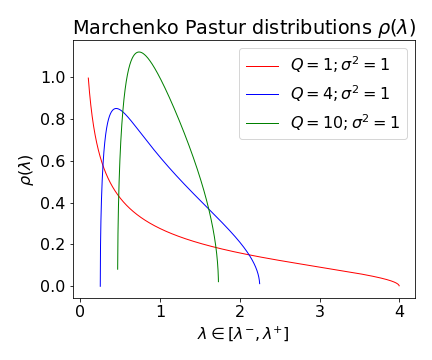
\includegraphics[width=7.0cm]{./img/mp-Q.png}
      \label{fig:MP-esds-a}
    }                               
    \subfigure[Tracy Widom fluctuations]{
      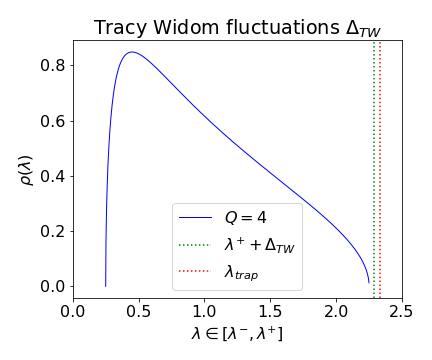
\includegraphics[width=7.0cm]{./img/mp-TW.png}
      \label{fig:MP-esds-b}
    }                    
    \caption{MP distributions for different aspect ratios $Q$ and variance scales $\sigma^2$, and an example of the finite-sized TW fluctuation $\Delta_{TW}$. }
   \label{fig:MP-esds}
\end{figure}

The Marchenko-Pastur (MP) distribution predicts the (limiting) \SHAPE of an ESD, $\rho_{MP}(\lambda)$, when the layer weight matrix has elements that are i.i.d. random from the Gaussian \Universality class.
%%As such, \HTSR theory is particularly useful when the ESD deviates from the MP predictions.
In particular, the ESD will be MP when the matrix elements are drawn from a Normal distribution $W_{i,j}\in  N(0,\sigma^{2})$, e.g., as is typical at initialization, before NN training begins.
Figure~\ref{fig:MP-esds} (from Figure~4 of \cite{MM18_TR_JMLRversion}) displays the MP distribution for different aspect ratios $Q=\tfrac{N}{M}$ and variances $\sigma^{2}$.  
Notice that the \SHAPE is characterized by a well defined, compact envelope with sharp edges.

The MP distribution also predicts the \SCALE of an ESD, again when the layer weight matrix has elements that are i.i.d. random from the Gaussian \Universality class.
In particular, an MP distribution, $\rho_{MP}(\lambda)$, has very crisp, well-defined lower and upper bounds $\lambda^{-},\lambda^{+}$~\cite{MM18_TR_JMLRversion}, and (importantly) the upper bound $\lambda^{+}$ exhibits finite-size Tracy-Widom (TW) fluctuations, $\Delta_{TW}(\lambda)$, which are on the order of $\mathcal{O}(M^{-2/3})$. 
Thus, any layer eigenvalue with \SCALE greater than this, i.e., $\lambda>[\lambda^{+}+\Delta_{TW}(\lambda)]$, is an ``outlier'' or a ``spike.''

According to the \HTSR \Phenomenology, these spikes carry significant generalizing information. 
(This is well-known for Bulk-Plus-Spike models~\cite{MM18_TR_JMLRversion}, but the \HTSR \Phenomenology generalizes this concept.)
%
Relatedly, for layer matrices $\mathbf{W}$ with aspect ratio $Q>1$ (i.e., rectangular matrices, where $N>M$), MP \RMT predicts there should be no zero eigenvalues, i.e., $\lambda_i>0$, for all $i$. 
Generally speaking, for well trained NNs, for layers with $Q>1$, all eigenvalues are strictly larger than zero, i.e., 
well-trained layer weight matrices, with $Q>1$, should have full rank and exhibit no ``rank collapse.'' 
\michael{MM TO DO: that sentence needs to go elsewhere.}
\HTSR places random Gaussian and ``Bulk-Plus-Spike'' matrices into the first two rows of Table~\ref{tab:Uclass}.
The essential feature of Gaussian random matrices is that their entries have no correlations. 
When some correlations are injected, a few large spike eigenvalues form, without otherwise disturbing the shape of the ESD. 
\michael{MM TO DO: put in comment about how bulk-plus-spike is just a perturbative variant of MP.}
To really understand how individual NN layers converge, we need to understand when and why their ESDs become HT.

%\chris{I cut a paragraph that only repeats things said elsewhere. \\
%These results are well-known within \RMT, but they have only recently been used as a diagnostic for NNs~\cite{MM18_TR_JMLRversion}.
%For example, if we randomize a well-trained layer matrix element-wise, $\mathbf{W}_{i,j}\rightarrow\mathbf{W}^{rand}_{i,j}$, i.e., if we permute the elements $W_{i,j}$, than we might expect the ESD of $\mathbf{W}^{rand}$ to fit an MP distribution; and it frequently does. 
%When it does not, the original ESD may have eigenvalues that are larger than the \SCALE of the TW fluctuation; and this may be due to (``real) correlations between pairs of data elements, and/or for other (``spurious) reasons.  
%These ``spurious correlations are often indicative of failures or suboptimalities of model training.
%In contrast, if we randomize a HT $\mathbf{W}$ row-wise (or column-wise), than the ESD will usually remain HT.
%}
%\charles{OK lets cut this}
%
%(Notice that if we randomize $\mathbf{W}$ column-wise or row-wise, however, the resulting ESD will retain most of its power law structure, and this will be ceritical later as we formulate the SETOL theory).


\subsubsection{\HeavyTailed \RandomMatrixTheory (\HTRMT) and \PowerLaw (PL) fits}
\label{sxn:htsr_pl_fits}

For very well-trained NN layers, ESDs are \emph{not} MP at all.
Frequently, if not always, their ESDs are HT---and they are HT \emph{because} they are strongly-correlated matrices.  
Importantly, they are \emph{not} HT element-wise.
Instead, their entries have a scale, and they have ESDs that are HT due to correlations learned during training. 
Existing theoretical approaches, including \SLT and even \STATMECH, cannot readily model such strongly-correlated systems.%
\footnote{For example, such theoretical approaches typically deal better with \emph{\Scale} information (such as $\lambda_{max}$) than with 
\emph{\Shape} information (such as $\alpha$), e.g., by characterizing an ``eigen-gap'' separating large eigenvalues from 
``noise''~\cite{bach2006_JMLR} according to a noise plus low-rank perturbation model~\cite{BFR11}.}

Such strongly-correlated systems, however, do frequently arise in other, related scientific domains, including
in the \STATMECH of self-organizing systems~\cite{bak97a,SornetteBook}, 
in electronic structure theory~\cite{Martin1996HighlyAA,martin_reparametrizing_1998,martin1996redesigning}, and
in quantitative finance~\cite{bouchaud1999,bouchaud2005,potters_bouchaud_2020}. 
In these (and other) domains, correlated systems frequently exhibit characteristic PL signatures; and it is common practice to \emph{model} correlated systems as random (uncorrelated) systems by using HT statistics (e.g., Levy distributions or PL random matrices), fully understanding that such systems are by no means actually i.i.d. random.
The \HTSR \Phenomenology builds upon this longstanding practice by 
%providing a qualitative \Phenomenology that characterizes the layers in well-trained NNs.
delimiting families of HT NN weight matrices based on the corresponding Universality classes of Pareto matrices. 

We explain briefly how to interpret Table~\ref{tab:Uclass} with respect to \HTRMT. The 5+1 Phases of Training can be 
identified by fitting ESDs to MP or PL distributions, whichever gives the best fit, as shown in the last column.
In case the PL distribution is a better fit, \HTSR \Phenomenology treats the layer weight matrix as 
equivalent to an i.i.d. random matrix $\mathbf{W}(\mu)$, whose elements have been drawn from a Pareto distribution 
with exponent $\mu$. 

\paragraph{Heavy-Tailed Universality Classes of Random Pareto Matrices}
For such an element-wise HT matrix, the theoretical \emph{limiting} ESD of a Pareto matrix is also PL,
which allows us to related the fitted PL $\alpha$ with exponent $\alpha=a\mu+b$, to the Pareto exponent $\mu$.
Ideally, for an infite width matrix ,  $a=\tfrac{1}{2}$ and $b=1$, but due to finite-size effects, however,
we have found we must take $a\ge \tfrac{1}{2}$ and $b\ge 1$, giving
\begin{align}
W_{i,j}(\mu)\sim\dfrac{C}{x^{\mu +1}},\;\;\;\rho(\lambda)\sim\lambda^{-(a\mu+b)}.
\end{align}
According to the above relation, 
we can use either the fitted PL exponent $\alpha$, or the Pareto exponent $\mu$,
to index the HT Universality classes,
Note, however, that the finite-size effects strongly depend on  the and aspect ratio  $Q=N/M$,
at least when applied to i.i.d random Pareto matrices, and 
the (Clauset MLE) PL fit may overestimate the $\alpha$ of the ESD.
Table~\ref{tab:Uclass} delimits the HT matrices 
into sub-categories (as shown in the bottom four rows)  based on the behaviors of $\alpha$ as a function of $\mu$.

Figure~\ref{fig:HT-esds} illustrates how the fitted PL exponent $\alpha$ corresponds to the actual Pareto exponent $\mu$ 
for different aspect ratios $Q=M/M$.a
Figure~\ref{fig:HT-esds-a} displays the ESDs of three different i.i.d. $1000\times1000$ HT random matrices, with $\mu=1,3,5$, on a Log-Log scale.  
Notice that smaller $\mu$, and therefore smaller $\alpha$, corresponds to heavier (i.e., larger) tails.
Figure~\ref{fig:HT-esds-b} shows how the empirically fit PL exponent $\alpha$ can vary with the theoretical $\mu$ for an associated $\mathbf{W}(\mu)$.
For $\mu<2$ and $Q=1$, the fitted $\alpha$ follows the linear relation $\alpha=\frac{1}{2}\mu+1$,
albeit with some error.
In contrast, for the more relevant $\mu \in (2,4)$ regime, the relation now depends far more 
strongly on the aspect ratio $Q$, and $\alpha\in[2,6]$.
For $\mu>4$, the fitted $\alpha$ saturates for each specific value of $Q$.

We emphasize that we only model the ESDs of the NN layer weight matrices using the
same Universality class to that an associated with the ESD of an random, i.i.d, HT Pareto matrix.
In fact, the elements $W_{i,j}$ do not at all appear as if they have been
drawn from a HT Pareto distribution, and, in contrast, are almost always well fit to a Laplacian distribution.
Also, despite these strong finite-size effects, empirically one finds that the ESDs arising large, well trained,
modern NNs can frequently be well fit  to a PL (or TPL), and that the fitted $\alpha\in [2,6]$ for $80-90\%$
of NN layers.  Notably, we rarely find $\alpha<2$ in the best performing, open source, pretrained DNNs.

\charles{Not sure where to put this..see text also}
%Despite the fact that Correlation-wise HT matrices found in NNs and Element-wise HT Pareto matrices arrive at their
As there is \emph{no} ground truth whatsoever as to the limiting spectral density of a strongly correlated NN weight matrix
(especially without HT elements)
the \HTSR \Phenomenology uses Pareto matrices as  a guide. 
However, as we will see in Section~\ref{sxn:HT_ESDs}, this analogy should be treated with caution because there are 
cases where it breaks down.

No matter why matrix ESD is HT, it can be difficult to reliably estimating the $\alpha$ parameter when
the true $\alpha$ is large. For Pareto matrices of the size investigated here, 
an observed $\alpha$ above $6$ is uninformative --- the tail will decay very rapidly indeed,
leaving very little of it to study.
In this sense, the HT Universality classes are \emph{larger} than the set of only strongly-correlated 
matrices or Pareto random matrices.



%and they can be used to model the strongly-correlated weight matrices $\mathbf{W}$---as long as we are careful to distinguish 
%between when $\mathbf{W}$ is element-wise HT and when $\mathbf{X}$ is correlation-wise HT. 
%HT because $\mathbf{W}$ is strongly-correlated.

\begin{figure}[h]
    \centering  
    \subfigure[Heavy Tailed ESDs]{ 
      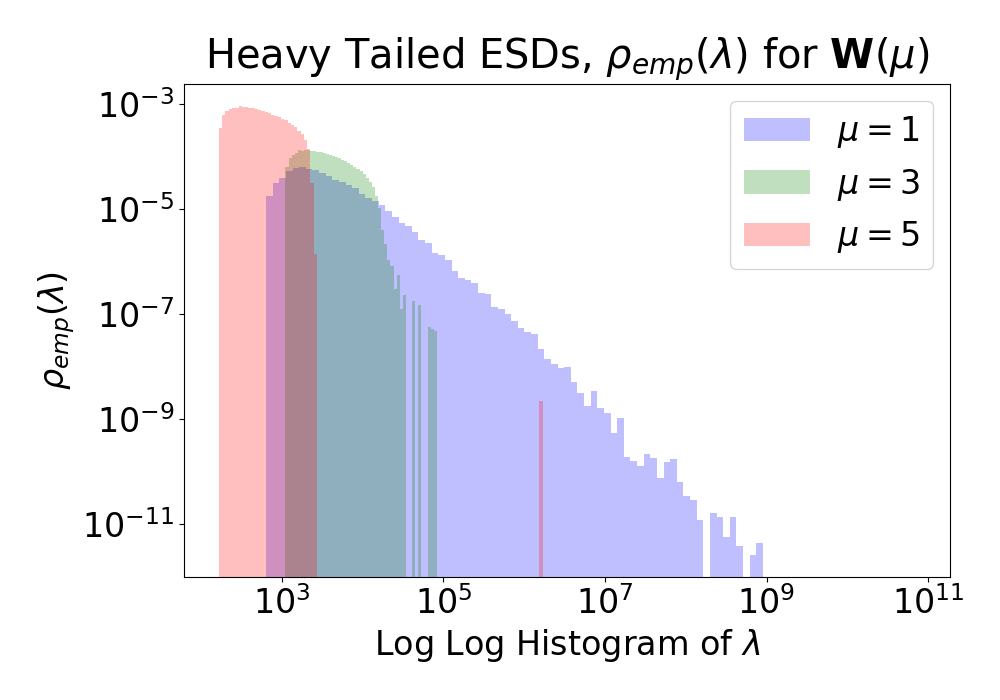
\includegraphics[width=7cm]{./img//heavy-tailed-log-log-esds.png}
      \label{fig:HT-esds-a}
    }                               
    \subfigure[PL $\alpha$ vs HT $\mu$ exponent]{
      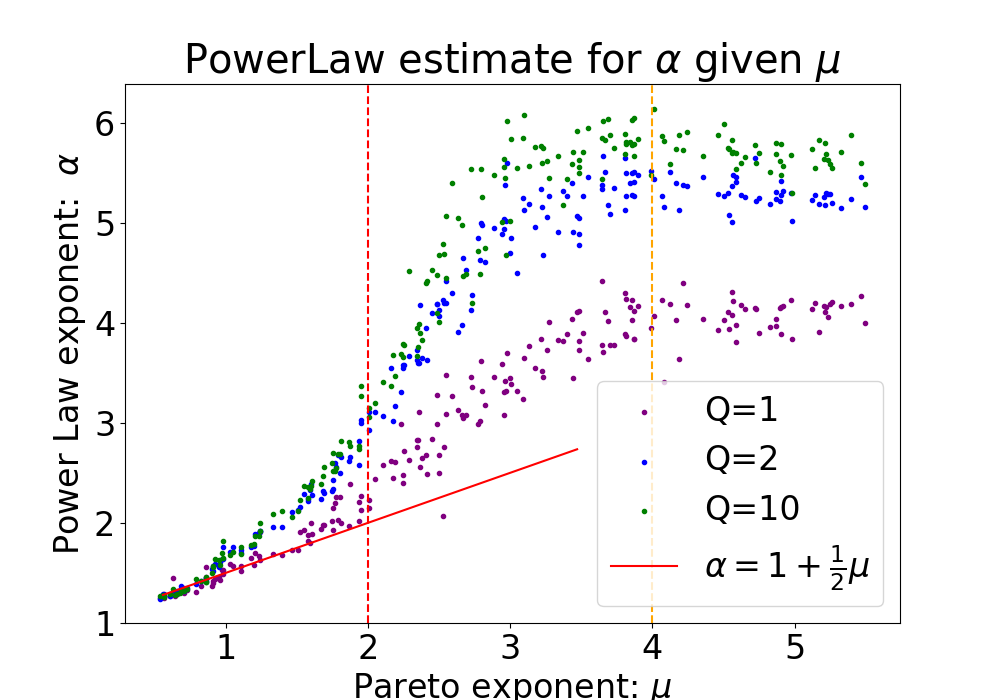
\includegraphics[width=7cm]{./img/alpha-mu-plot2.png}
      \label{fig:HT-esds-b}
    }                                                                                                                            
    \caption{Comparison of ESDs and Power Law (PL) exponents $\alpha$ from Heavy-Tailed (Pareto) 
weight matrices $\mathbf{W}(\mu)$. 
Subfigure (a) depicts 3 \Typical ESDs with Pareto exponent $\mu=1,3,5$, each decreasing in \SHAPE~and \SCALE.
Subfigure (b) shows how the exponent $\alpha$ of the PL fit varies with $\mu$, with significant finite-size
effects emerging for $\mu>2$ and $\alpha>2$.
}
   \label{fig:HT-esds}
\end{figure}

There is a particularly important boundary between Universality classes where $\alpha = 2$. Recall that one of the 
properties of power law distributions $\rho(\lambda)\sim \lambda^{-\alpha}$ is that if $\alpha<2$, than the variance of 
$\rho(\lambda)$ is infinite. In such cases, the variance cannot be estimated empirically, making $\rho(\lambda)$ in 
some sense \emph{\ATypical}. This implies that the NN will have substantially greater difficulty in applying any further 
load to such a weight matrix. Thus, the value of $\alpha = 2$ is a \emph{critical value}. (See 
Figure~\ref{fig:mlp3-FC1-alpha-overloaded} in Section~\ref{sxn:hysteresis_effect} for an empirical study of this effect 
in a small MLP.)

%When fitting ESDs of well-trained models, 
Smaller PL exponent $\alpha$ values correspond to heavier tails, $\rho_{tail}(\lambda)$; and
the \HTSR \Phenomenology observes that smaller PL exponents $\alpha$ (at least for $\alpha\in(2,6)$) tend to correspond to better models.
This is the key idea of the \HTSR:
the generalizing components of a layer matrix $\mathbf{W}$ concentrate in larger singular vectors associated with the tail, and 
so that better models have more slowly-decaying (i.e., larger) ESD tails.
This differs significantly than simply taking a general low-rank approximation to $\mathbf{W}$, where the rank
is chosen without insight from the \HTSR \Phenomenology. 
The \SETOL theory formalizes this observation as a key assumption. We will revisit these model selection questions in 
Section~\ref{sxn:setol_overview} below.
\michael{This par seems to contain a main point. It should probably be above.}


